\documentclass[conference]{IEEEtran}

\usepackage[utf8]{inputenc}
\usepackage[T1]{fontenc}
\usepackage[brazil]{babel}
\usepackage{graphicx}
\usepackage{amsmath}
\usepackage{booktabs}
\usepackage{cite}
\usepackage{url}
\graphicspath{{results/report/}}

\title{AnimalSight: Avaliação de Regiões de Interesse\\
na Classificação de Raças de Cães}

\author{
\IEEEauthorblockN{João Meyer Muhlmann}
\IEEEauthorblockA{Universidade Federal do Paraná\\
Trabalho Final de Visão Computacional\\
Novembro de 2026}
}

\begin{document}
\maketitle

\begin{abstract}
Este trabalho investiga se uma região de interesse (ROI), selecionada
por processamento clássico de imagens, melhora a classificação de
raças de cães em resoluções reduzidas. O AnimalSight combina o DINOv2
congelado com um classificador SVM e compara o processamento convencional
com um recorte baseado em gradientes Sobel. Foram utilizadas cinco raças
do Oxford-IIIT Pet, com 500 imagens de treinamento e 499 de teste.
A entrada de 112\,$\times$\,112 pixels alcançou 99,40\% de acurácia,
frente a 100,00\% em 224\,$\times$\,224, com ganho de velocidade de
$2{,}61\times$ na CPU utilizada. A ROI atingiu 97,39\% em 112 pixels
e permaneceu abaixo do redimensionamento convencional em todas as
resoluções avaliadas. Embora tenha corrigido erros individuais, ela
introduziu mais erros do que corrigiu. Os resultados motivam o estudo
de métodos que delimitem melhor o animal antes da redução.
\end{abstract}

\begin{IEEEkeywords}
visão computacional, região de interesse, DINOv2, SVM.
\end{IEEEkeywords}

\section{Introdução}
A classificação de raças de cães depende de características como
formato da cabeça, orelhas, pelagem e proporções do corpo. Ao reduzir
uma imagem, parte desses detalhes pode desaparecer. Por outro lado,
processar imagens menores pode diminuir o tempo de inferência, o que
motiva investigar o compromisso entre custo computacional e acurácia.

O DINOv2 fornece características visuais que podem ser reutilizadas
em tarefas de reconhecimento sem ajustar os pesos do extrator~\cite{dinov2}.
Isso permite estudar diferentes formas de preparar a imagem mantendo
o mesmo modelo pré-treinado. Neste trabalho, a aprendizagem supervisionada
fica restrita a um SVM, treinado sobre os vetores produzidos pelo DINOv2.

A hipótese investigada é que selecionar uma região de interesse antes
de reduzir a imagem poderia preservar mais detalhes do animal, pois
uma parcela maior dos pixels disponíveis seria dedicada a ele.
Entretanto, esse benefício depende de o recorte selecionar a região
correta: uma área com muitos contornos também pode pertencer ao fundo.

O objetivo do AnimalSight é comparar três alternativas: a entrada
de referência em 224 pixels, a redução convencional e a redução após
seleção de ROI por gradientes. Além da comparação em 112 pixels,
avaliam-se resoluções progressivamente menores para verificar se a ROI
se torna vantajosa quando há maior perda de informação visual.

\section{Metodologia}
\subsection{Conjunto de dados}
Utilizaram-se cinco raças do Oxford-IIIT Pet~\cite{pets}: beagle,
boxer, chihuahua, samoyed e yorkshire terrier. Mantiveram-se as divisões
oficiais: 500 imagens de treinamento, sendo 100 por raça, e 499 de
teste, sendo 99 de boxer e 100 de cada uma das demais raças.
As mesmas imagens foram utilizadas em todas as configurações.

O problema é de classificação entre essas cinco classes. O sistema
não foi treinado para localizar vários animais nem para rejeitar
objetos ou raças ausentes do treinamento. Embora o conjunto disponibilize
anotações de localização e segmentação~\cite{pets}, elas não foram
utilizadas para construir a ROI deste experimento.

\subsection{Configurações e pré-processamento}
O \textit{Baseline} recebe uma entrada de 224\,$\times$\,224 pixels.
O \textit{Reduced} aplica o mesmo processamento à imagem original,
com uma resolução menor. O \textit{ROI Reduced} seleciona primeiro
um recorte quadrado e aplica a ele o processamento do Reduced.
Assim, a comparação entre Reduced e ROI Reduced mantém a mesma
resolução de entrada e altera a região da imagem utilizada.

Após a seleção opcional da ROI, a imagem é convertida para RGB,
redimensionada com interpolação bicúbica, recortada no centro e
normalizada conforme o processador do DINOv2. Para uma entrada de
lado $r$, a menor dimensão é redimensionada para
$\lfloor 256r/224 \rfloor$, seguida de recorte central $r\times r$.
Portanto, o Reduced também realiza o recorte central convencional;
a diferença da ROI está na seleção prévia de uma região por gradientes.

Foram avaliados $r\in\{112,84,56,42,28\}$, mantendo a escala da ROI
em 0,8. Com o baseline, isso totaliza 11 configurações.

\subsection{Seleção clássica da ROI}
A imagem é convertida para tons de cinza e suavizada por um filtro
gaussiano de $5\times5$, com $\sigma=1$. Calculam-se as derivadas
horizontais e verticais com Sobel e a magnitude
$\sqrt{G_x^2+G_y^2}$. Um segundo filtro gaussiano, de $15\times15$,
suaviza esse mapa, produzindo $M$.

Para uma imagem de largura $W$ e altura $H$, define-se uma janela
quadrada de lado $s=\max(1,\lfloor0{,}8\min(H,W)\rfloor)$.
A região escolhida é
\begin{equation}
R^*=\underset{R\in\mathcal{R}_s}{\operatorname{arg\,max}}
\sum_{(x,y)\in R} M(x,y),
\end{equation}
em que $\mathcal{R}_s$ contém todas as posições válidas dessa janela.
Na implementação, um filtro de soma calcula os escores das regiões.

O método procura uma área com alta concentração de bordas, sem
reconhecer semanticamente o animal. Ele não utiliza rótulos, máscaras
ou um detector aprendido. Sua simplicidade facilita o experimento,
mas não garante que cabeça e corpo permaneçam dentro do recorte.

\subsection{Extração de características e classificação}
O modelo \texttt{facebook/dinov2-small} permanece congelado durante
todo o processo. O token CLS da última camada representa cada imagem
por um vetor de 384 características. Um \texttt{StandardScaler},
ajustado apenas no treinamento, padroniza os vetores, que alimentam
um SVM com kernel RBF, $C=10$ e \texttt{gamma=scale}.

Cada configuração utiliza um SVM próprio, treinado nas mesmas 500
imagens. Isso permite que o classificador se adapte à representação
produzida por cada resolução e estratégia de recorte. Os parâmetros
do SVM permanecem fixos em todas as comparações.

Como o modelo utiliza patches de $14\times14$ pixels, a quantidade
de tokens, incluindo o CLS, é $N(r)=1+(r/14)^2$ nas resoluções adotadas.
São 257 tokens em 224 pixels, 65 em 112 e apenas cinco em 28.
A redução altera efetivamente a entrada do transformer, enquanto a
dimensão do vetor de características e os pesos do DINOv2 permanecem iguais.

\subsection{Métricas e medição de tempo}
A avaliação considera a acurácia e o F1 macro, que atribui o mesmo
peso a cada raça. Também são contadas, imagem por imagem, as situações
em que a ROI corrige um erro do Reduced ou transforma um acerto em erro.

O tempo foi medido em uma CPU Intel Core i7-1065G7, com quatro threads,
lote unitário e duas passagens pelas 499 imagens: 998 medições por
configuração. Cada passagem inclui cinco inferências de aquecimento
por configuração, excluídas das medidas. A ordem das imagens e das
configurações é aleatorizada com semente 42.

A medição inclui pré-processamento, ROI quando aplicável, DINOv2 e SVM;
exclui leitura e decodificação dos arquivos, carregamento dos modelos
e treinamento. Embeddings em cache são utilizados para facilitar a
reexecução do experimento, mas não para medir a inferência.

\section{Resultados e Discussão}
\subsection{Comparação principal}
A Tabela~\ref{tab:principal} apresenta os resultados em 224 e 112 pixels.
O baseline acertou as 499 imagens. O Reduced acertou 496, alcançando
99,40\% de acurácia, com perda de apenas 0,60 ponto percentual.
Seu tempo médio caiu de 217,01 para 83,20 ms por imagem, correspondendo
a um ganho de velocidade de $2{,}61\times$.

O ROI Reduced acertou 486 imagens e atingiu 97,39\% de acurácia.
Seu tempo médio foi de 72,18 ms. Como as duas alternativas em 112 pixels
utilizam 65 tokens, esse tempo menor não demonstra, por si só, uma
vantagem computacional da ROI. Houve dispersão nas medidas: os desvios
padrão foram 53,96, 53,75 e 26,00 ms para baseline, Reduced e ROI Reduced,
respectivamente. Os tempos descrevem esta execução no equipamento utilizado.

Além disso, reduzir a entrada não comprime o modelo: os pesos do DINOv2
são compartilhados e mantêm o mesmo tamanho. O ganho observado está
no tempo de processamento, com pequena perda de acurácia no Reduced 112.

\begin{table}[t]
\caption{Comparação nas 499 imagens de teste. Tempo médio por imagem;
ganho relativo ao baseline. Reduced e ROI Reduced utilizam 112 pixels.}
\label{tab:principal}
\centering
\footnotesize
\setlength{\tabcolsep}{4pt}
\begin{tabular}{lrrrr}
\toprule
Configuração & Acc. (\%) & F1 macro & Tempo (ms) & Ganho \\
\midrule
Baseline    & 100,00 & 1,0000 & 217,01 & $1{,}00\times$ \\
Reduced     & 99,40  & 0,9940 & 83,20  & $2{,}61\times$ \\
ROI Reduced & 97,39  & 0,9740 & 72,18  & $3{,}01\times$ \\
\bottomrule
\end{tabular}
\end{table}

\subsection{Efeito de reduções mais intensas}
A Tabela~\ref{tab:resolucoes} e a Fig.~\ref{fig:resolucoes} mostram
que diminuir ainda mais a entrada intensifica a perda de acurácia.
O Reduced mantém 96,19\% em 84 pixels, mas cai para 75,55\% em 56,
64,33\% em 42 e 57,11\% em 28. A passagem de 84 para 56 pixels
representa uma queda de 20,64 pontos percentuais.

A ROI não supera o Reduced em nenhuma resolução. A menor diferença
observada ocorre em 56 pixels: 74,75\% contra 75,55\%, uma desvantagem
de 0,80 ponto percentual. Em 28 pixels, a diferença aumenta para
3,01 pontos percentuais. Portanto, a maior redução da imagem não
tornou esta estratégia de ROI vantajosa em acurácia global.

\begin{table}[t]
\caption{Acurácia por resolução e efeito da ROI sobre as previsões do
Reduced. Corrige: erro que vira acerto; piora: acerto que vira erro.}
\label{tab:resolucoes}
\centering
\footnotesize
\setlength{\tabcolsep}{4pt}
\begin{tabular}{crrrr}
\toprule
Lado (px) & Reduced (\%) & ROI (\%) & Corrige & Piora \\
\midrule
112 & 99,40 & 97,39 & 1  & 11 \\
84  & 96,19 & 94,99 & 10 & 16 \\
56  & 75,55 & 74,75 & 52 & 56 \\
42  & 64,33 & 61,92 & 59 & 71 \\
28  & 57,11 & 54,11 & 72 & 87 \\
\bottomrule
\end{tabular}
\end{table}

\begin{figure}[t]
\centering
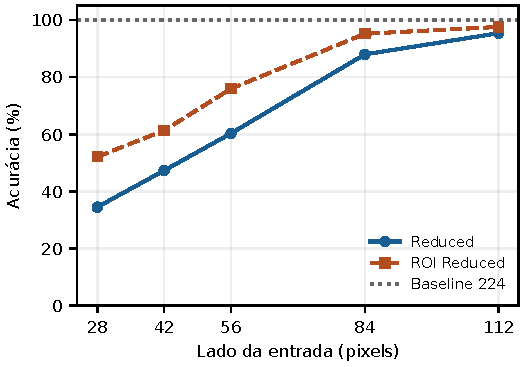
\includegraphics[width=\columnwidth]{accuracy_vs_resolution.pdf}
\caption{Acurácia nas resoluções reduzidas. A linha pontilhada indica
o resultado do baseline em 224 pixels.}
\label{fig:resolucoes}
\end{figure}

\subsection{Quando a ROI ajuda ou prejudica}
A ausência de ganho global não significa que o recorte prejudique
todas as imagens. Em 112 pixels, a ROI corrige um erro do Reduced,
mas introduz 11. Em 28 pixels, corrige 72 e introduz 87, produzindo
um saldo de 15 acertos a menos. Esses números explicam por que
existem exemplos favoráveis à ROI mesmo quando a média é inferior.

A Fig.~\ref{fig:casos} apresenta dois casos de teste em 112 pixels.
Em \texttt{samoyed\_91}, o Reduced prevê boxer e a ROI recupera a classe
samoyed. Em \texttt{beagle\_30}, o Reduced acerta beagle e a ROI prevê
boxer; nesse exemplo, a ROI deixa a cabeça do animal fora da entrada.
Os casos foram selecionados pelas diferenças nas previsões
para ilustrar os dois comportamentos, não para estimar sua frequência.

Uma hipótese para as perdas é que a soma de gradientes favoreça
texturas e contornos sem distinguir o animal do cenário. Além disso,
a janela quadrada fixa pode retirar partes discriminativas ou alterar
a proporção entre cabeça, corpo e contexto. A comparação mostra o
efeito final do processamento, mas não isola qual dessas causas
explica cada erro.

\begin{figure}[t]
\centering
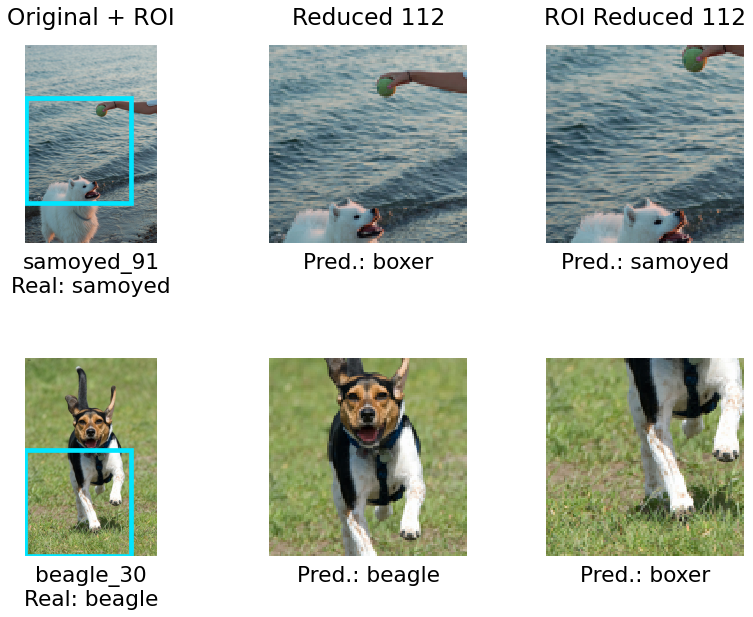
\includegraphics[width=\columnwidth]{roi_cases.png}
\caption{Exemplos do conjunto Oxford-IIIT Pet~\cite{pets} em que a ROI
corrige um erro (acima) e introduz um erro (abaixo). O retângulo indica
a ROI inicial; as outras colunas mostram as entradas efetivas em
112 pixels, com a normalização desfeita para visualização.}
\label{fig:casos}
\end{figure}

\subsection{Limitações}
O estudo é exploratório e utiliza cinco raças, um extrator congelado
e uma única estratégia de ROI. As comparações reutilizam o mesmo
conjunto oficial de teste. Assim, os 100\% do baseline se referem
às 499 imagens avaliadas e não garantem desempenho equivalente em
fotografias externas ou em outras raças.

As medições de tempo abrangem apenas 224 e 112 pixels; não permitem
quantificar o ganho de velocidade das resoluções menores. Também
não foi estabelecida significância estatística para as diferenças
observadas. Os resultados sustentam a comparação neste experimento,
sem demonstrar que toda seleção de ROI seja inferior.

\section{Conclusão e Trabalhos Futuros}
A redução convencional para 112\,$\times$\,112 apresentou uma relação
favorável entre acurácia e tempo de inferência: 99,40\% de acertos e
ganho de $2{,}61\times$ em relação ao baseline. Reduções mais intensas
diminuíram a acurácia, especialmente abaixo de 84 pixels.

A hipótese de que a ROI por gradientes compensaria essa perda não
se confirmou. O recorte ajudou algumas imagens, mas introduziu mais
erros do que corrigiu em todas as resoluções. Para a configuração
estudada, o Reduced 112 é a alternativa mais adequada quando se busca
diminuir o tempo mantendo a acurácia próxima à referência.

Como trabalho futuro, propõe-se melhorar a delimitação do animal,
combinando gradientes com segmentação de primeiro plano e operações
morfológicas. Recortes de tamanho e formato adaptativos podem ajudar
a preservar a cabeça e o corpo. As anotações de localização e
segmentação do Oxford-IIIT Pet~\cite{pets} também podem servir como
referência para medir a qualidade da região selecionada, separadamente
da classificação.

Outra possibilidade é comparar a ROI por gradientes com um recorte
central de mesmo tamanho, isolando melhor o efeito da posição
escolhida. Qualquer melhoria deve considerar tanto a acurácia quanto
o tempo adicional de pré-processamento, pois um recorte melhor só
atende ao objetivo se mantiver um custo de inferência adequado.

\begin{thebibliography}{2}

\bibitem{dinov2}
M. Oquab \textit{et al.}, ``DINOv2: Learning Robust Visual Features
without Supervision,'' arXiv:2304.07193, 2023.
\url{https://arxiv.org/abs/2304.07193}

\bibitem{pets}
O. M. Parkhi, A. Vedaldi, A. Zisserman e C. V. Jawahar,
``Cats and Dogs,'' in \textit{Proc. IEEE Conference on Computer Vision
and Pattern Recognition (CVPR)}, 2012.
\url{https://www.robots.ox.ac.uk/~vgg/data/pets/}

\end{thebibliography}
\end{document}
